\chapter{Umsetzung und Implementierung}

\todo[inline]{Sinnvoller einstiegstext in das Kapitel}


\section{Software}

\color{blue}
\begin{itemize}
    \item Virtual Python environment.
    \item Implementiert in TensorFlow. (angefangen in version 1.8, später nach 1.11 upgedatet)
    \item tensorflow-gpu - .
    \item Datenhandling: mit Pandas. Da Data Science ein wichtiger Part der Arbeit war, sehr wichtig erwähnen
    \item Matplotlib für Visualisierung (die meisten selbstgemachten grafiken hier in der Arbeit)
    \item OpenCV für Bilderdinge in der Pipeline (wie oben erwähnt)
    \item MATLAB, für Tracksort und die Ursprünglichen implementation der Vergleichsdinge für evaluationen 
\end{itemize}
\color{black}

Für die Umsetzung der neuronalen Netze wurde im Rahmen dieser Arbeit 
das Open Source Framework TensorFlow\footnote{https://www.tensorflow.org/} verwendet.
Es wurde die \texttt{tensorflow-gpu} Variante mittels pip in einem Python~3.6.5 virtual environment installiert.
Zu Beginn der Arbeit wurde die zum damaligen Zeitpunkt aktuelle TensorFlow Version 1.8 installiert 
und zu einem späteren Zeitpunkt wurde auf Version~1.11 geupdatet, die bis zum Ende verwendet wurde.

Weitere wichtige Software, die verwendet wurde 
sind \textit{pandas} in der Version~0.23.1, was für den Umgang mit den Daten genutzt wurde, 
und \textit{matplotlib} in der Version~3.0.0, mit dem die Visualisierung der Ergebnisse und die meisten Grafiken dieser Arbeit generiert wurden.
Desweiteren wurde die Python Bindings von \textit{OpenCV} für die Verarbeitung der aufgenommen Bilder verwendet.
Der existierende \textit{Predictive Tracking} Algorithmus ist in \textsc{Matlab} implementiert, 
weshalb einige Teile der Arbeit auch das verwenden.

% \todo[inline]{Aufpassen dass das nicht zu viel wird}

\section{Code Struktur}

Vorgehen beschrieben in \ref{CodeStruktur}.
\todo[inline]{überlegen wie viel ich überhaupt dazu schreiben soll - }

\begin{figure}[h]
    \centering
    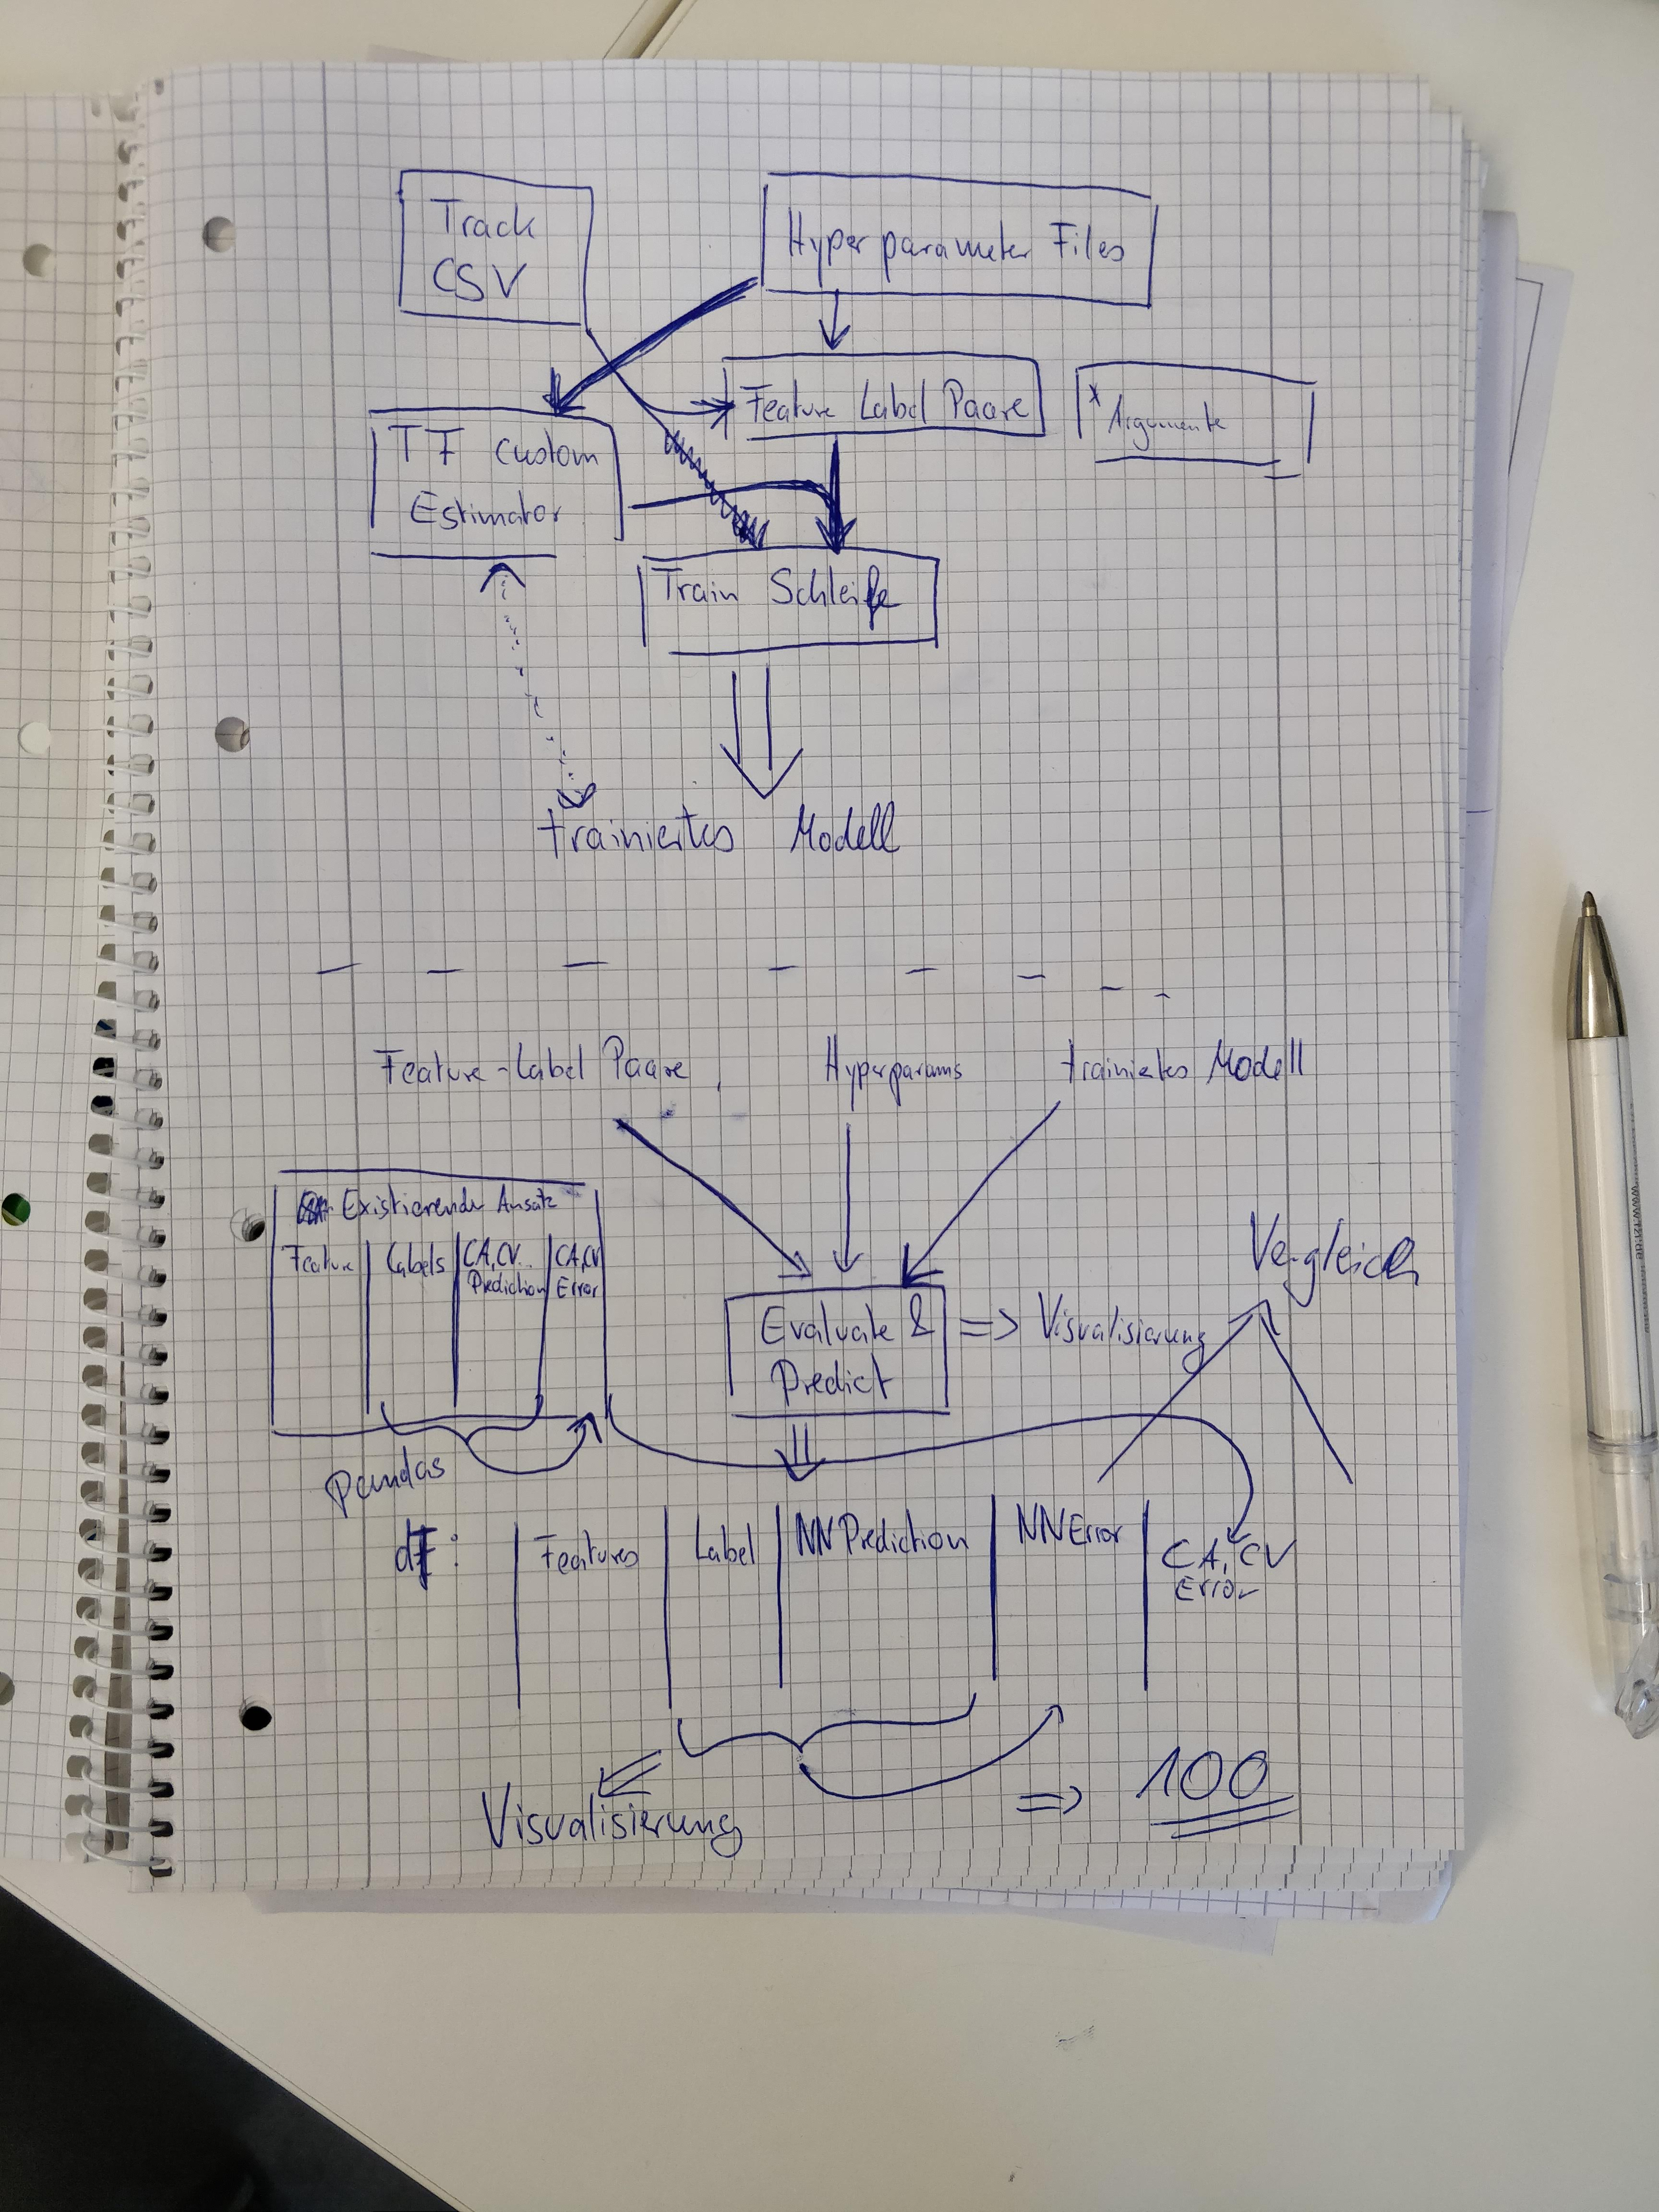
\includegraphics[width=\textwidth]{CodeStrukturSkizze}
    \caption{Skizze Codestruktur}
    \label{CodeStruktur}
\end{figure}
  

\section{Hyperparameter}

\color{blue}
Hyperparameter sind die Variablen, die die Struktur des Netzes bestimmen (Eg: Anzahl Layers, FeatureSize) 
sowie die Variablen, die festlegen wie das Netz trainiert (z.B. Lernrate, Anzahl Epochen)
Hyperparameter werden vor dem Beginn des Trainings festgelegt und bleiben während dem kompletten Training unverändert.
Vorgehen bei dieser Arbeit: Jeweils für NextStep und für Separator getrennte Konfigurationen finden.
\color{black}

Im Kontext des maschinellen Lernens bezeichnet man jene Variablen als Hyperparameter, 
die bereits vor dem Beginn des Trainings festgelegt sein müssen.
Beispiele für solche Hyperparameter sind zum Beispiel Aspekte der Netzarchitektur, wie die Anzahl der Layers und ihre jeweilige Größe 
oder speziell im Falle dieser Arbeit die \textit{FeatureSize}, die festlegt, welche Form der Input des Netzes annimmt.
Auch Parameter, die festlegen wie das Netz lernt - also Lernrate oder die Anzahl der Epochen beim Training - zählen dazu.

Die Implementierung dieser Arbeit hat die Definition der Hyperparameter aus dem Programmcode selbst ausgelagert.
Stattdessen können sogenannte Hyperparameter Dateien im JSON Dateiformat definiert werden, die dann vom Programm geladen werden.
Dies vereinfacht das Training und das Testen von Netzen mit unterschiedlichen Hyperparametern, 
wie es bei Netzen des NextStep Typs und des Separator Typs der Fall ist.
Einzelne Parameter aus den Dateien können per Kommandozeilenparameter überschrieben werden.
Ein Beispiel für eine solche Hyperparameter Datei ist Listing~\ref{lst-hyperparam} zu sehen.
Die Bedeutung der einzelnen Parameter soll im folgenden erklärt werden.


\noindent\begin{minipage}{\textwidth}
\begin{lstlisting}[language=json,firstnumber=1, caption={Beispiel einer Hyperparameter Datei in JSON}, captionpos=b, label=lst-hyperparam]

    {
        "arch": {
            "dropoutRate": 0.0,
            "hiddenLayers": [16, 16, 16],
            "featureSize": 5,
            "activation": "leaky_relu",
            "regularization": "no"
        },
        "problem": {
            "dataPath": "/home/hornberger/MasterarbeitTobias/data/selbstgesammelteDaten2/Kugeln-Band-Juli/",
            "modelBasePath": "/home/hornberger/MasterarbeitTobias/models/real/NextStep/NextStep-45kDecaySteps-SpheresReal",
            "imagePath": "/home/hornberger/MasterarbeitTobias/images/Real-NextStep-45kDecay-Spheres",
            "separator": 0,
            "separatorPosition": 1550,
            "thresholdPoint": 1200,
            "predictionCutOff": 1500

        },
        "train": {
            "batchSize": 500,
            "epochs": 3000,
            "stepsPerEpoch": 5000,
            "learningRate": 0.005,
            "decaySteps": 45000,
            "optimizer": "Adam"
        },
        "data": {
            "testSize": 0.1,
            "augmentMidpoint": 1123,
            "augmentRange": 1000,
            "direction": "x",
            "unitLoc": "px",
            "unitTime": "1/100 Frames",
            "limits": [0, 2350, 0, 1750]
        }
}



    
\end{lstlisting}
\end{minipage}
    
% \begin{itemize}
% \item Architektur:
%     \begin{itemize}
%         \item Dropout: Wahrscheinlichkeit für das zufälliges ausschalten von einzelnen Neuronen
%         \item Hidden Layer: ein Array an Zahlen repräsentiert die Architektur der Hidden Layers. Jede Zahl ist ein FC Layer mit so vielen neuronen
%         \item FeatureSize: Wie viele Positionen bekommt das Netz als Input ( \textrightarrow{} Größe des Inputlayers = 2x FeatureSize)
%         \item Activation: Aktivierungsfunktionen für die neuronen der Hidden Layers
%         % - optionen: "relu", "leaky_relu", "linear"
%     \end{itemize}
% \item Problem:
%     \begin{itemize}
%         \item DataPath: wo liegen die CSV Dateien zum die Daten rausladen
%         \item ModelPath: wo soll das Netz hingespeichert werden/Hergeladen - mit Checkpoints usw.
%         \item ImagePath: wo sollen Bilder hingespeichert werden, z.B. von Plot
%         \item separator: 0 oder 1, jenachdem ob es den nächsten Schritt (0) oder zum Düsenbalken (1) prädizieren soll
%     \end{itemize}

%     Falls Separator 1:
%     \begin{itemize}
%         \item separationPosition: Koordinate des Düsenbalken und Ziel der Prädiktion
%         \item ThresholdCutoff \todo{verify}
%         \item predictionCutOff: Koordinate hinter der keine FeatureTupel mehr genommen werden
%     \end{itemize}
% \item Train:

% \end{itemize}

% \begin{description}[align=right]
%     \item [Kate] some detail
%     \item [Christina]some detail
%     \item [Laura]some detail
% \end{description}

% \begin{itemize}
    % \item Architektur:
    
\bigskip
{\Large \sffamily \textbf{arch}}
\begin{description}[leftmargin=!,labelwidth=\widthof{\bfseries separatorPosition}, labelindent=0.5cm]
    \item [dropoutRate] Wahrscheinlichkeit für das zufälliges Ausschalten von einzelnen Neuronen beim Training, entsprechend der Beschreibung in Unterabschnitt~\ref{ssec:Regul}.
    \item [hiddenLayers] Ein Array an Zahlen, das die Architektur der Hidden Layers repräsentiert. Jede Zahl steht für ein FC Layer mit der entsprechenden Anzahl Neuronen.
    \item [featureSize] Anzahl der vergangen Positionen, die das Netz als Eingabe bekommt.
    \item [activation] Legt die Aktivierungsfunktionen für die Neuronen der Hidden Layers fest. Valide Werte sind ReLU, Leaky ReLU und lineare Aktivierungsfunktionen.
    % - optionen: "relu", "leaky_relu", "linear"
\end{description}

\bigskip
{\Large \sffamily \textbf{problem}}

\begin{description}[leftmargin=!,labelwidth=\widthof{\bfseries separatorPosition}, labelindent=0.5cm]
    \item[dataPath] Ort im Dateisystem, wo die CSV Dateien mit den Track Informationen liegen.
    \item[modelBasePath] Ort im Dateisystem, an dem das Modell des Netzes und alle damit verbundenen Dateien gespeichert wird, beziehungsweise woher es geladen wird. 
    \item [imagePath] Ort im Dateisystem, wo sollen Schaubilder, Visualisierungen oder Ähnliches gespeichert werden sollen.
    \item [separator] Hyperparameter, der festlegt, welcher Typ von Netz trainiert werden soll. Ob es den nächsten Schritt (0) oder zum Düsenbalken (1) prädizieren soll.
\end{description}

% Falls Separator 1:
\begin{description}[leftmargin=!,labelwidth=\widthof{\bfseries separatorPosition}, labelindent=0.5cm]
    \item[separatorPosition] Koordinate des Düsenbalken und Ziel der Prädiktion entlang der Bewegungsrichtung des Förderbands
    \item[thresholdPoint] Koordinate des Punkts ab dem prädiziert wird.
    \item[predictionCutOff] Koordinate des Punkts ab dem die Tracks abgeschnitten werden um privilegierte Information zu vermeiden.
\end{description}

\bigskip
{\Large \sffamily \textbf{train}}

\begin{description}[leftmargin=!,labelwidth=\widthof{\bfseries separatorPosition}, labelindent=0.5cm]
    \item[batchSize] Die Anzahl der Feature-Label-Paare, die in einer Iteration betrachtet werden.
    \item[epochs] Die Anzahl der Epochen für die trainiert wird.
    \item[stepsPerEpoch] Die Anzahl der Iterationen, die in einer Epoche durchgeführt werden.  
    \item[learningRate] Anfängliche maximale Lernrate, mit der die Gewichte geändert werden
    \item[decaySteps] Parameter, der festlegt wie schnell die maximale Lernrate reduziert wird. 
    \item[optimizer] Der Optimizer, der fürs Training verwendet wird.
\end{description}

\bigskip
{\Large \sffamily \textbf{data}}
% \item Data:
\begin{description}[leftmargin=!,labelwidth=\widthof{\bfseries separatorPosition}, labelindent=0.5cm]
    % \item[numberFakeLines] Anzahl der synthetischen Trainingsbeispiele, die generiert werden sollen.
    \item[testSize] Parameter, der die Aufteilung zwischen Trainings- und Testdaten festlegt. Ein Wert von 0.1 würde einen 90:10 Split Training zu Test bedeuten.  
    \item[augmentMidpoint] Koordinate, der Spiegelachse an der für die Data Augmentation gespiegelt wird.
    \item[augmentRange] Breite des Bandes, zu einer Seite, in dem die Spiegelung angewendet werden soll. Feature-Label-Paare mit einem Element außerhalb des Bandes werden ignoriert.
    \item[direction] Bewegungsrichtung der Partikel. ``x'' bei simulierten Daten, ``y'' bei Selbstgesammelten.
    \item[unitLoc] Einheit des Orts. ``m'' beziehungsweise Meter bei simulierten Daten, ``px'' beziehungsweise Pixel bei Selbstgesammelten.
    \item[unitTime] Einheit der Zeit. 
    \item[limits] Bereich, der in der Visualisierung dargestellt wird. [0.388, 0.788, 0, 0.18] bei simulierten Daten,  [0, 2350, 0, 1750] bei Selbstgesammelten.

\end{description}
% \end{itemize}



\subsection{Hyperparameter Tuning}

Als Hyperparameter Optimierung oder auch Hyperparameter Tuning bezeicht man den Vorgang das am besten geeignete Set an 
Hyperparametern für einen Lernalgorithmus zu wählen.



Vorgehen um optimale Hyperparameter zu finden: 
Baseline wird (über den Daumen gepeilt).
Training mehrere Modelle mit variierenden Werten für einen einzelnen Parameter, 
während die restlichen Parameter unverändert bleiben.

So viele modelle zu trainieren ist sehr zeitintensiv, deshalb:
Suchen auf Simulierten Daten (Spheres) und dann auf allen Daten verwenden.

Nicht optimal... Maybe ausblick?


Aktueller Stand:
NextStep: kein Overfitting gefunden \textrightarrow L1 und L2 Regularisierung haben keinen positiven Effekt.\\
Adam Optimizer ist am besten. \todo{erklären was genau der Adam optimizer eigentlich macht} \\
leaky\_relu reigns supreme. \\
Learning Rate Decay ist eine gute Idee. (Höherer Wert \textrightarrow langsamerer Zerfall). \\
FeatureSize 5 ist gut, weniger wird schlechter und Mehr ist auch schlechter geworden (potenziell weil weniger Beispiele?)
Dropout macht es kaputt, also auf 0.0 setzen

Separator: 

\subsection{Architektur des neuronalen Netzes}

Input layer: \(2 * FeatureSize\) Neuronen

\(N\) hiddenlayer (as determined by Hyperparameter tuning) mit jeweils \(m\) Neuronen.
Fully connected!

Output layer:
Linear activation weil regression.
2 Neuronen, eins für die eine Label Dimension und eins für die andere.

\begin{figure}[h]
    \centering
    % \missingfigure{Grafik architektur}
	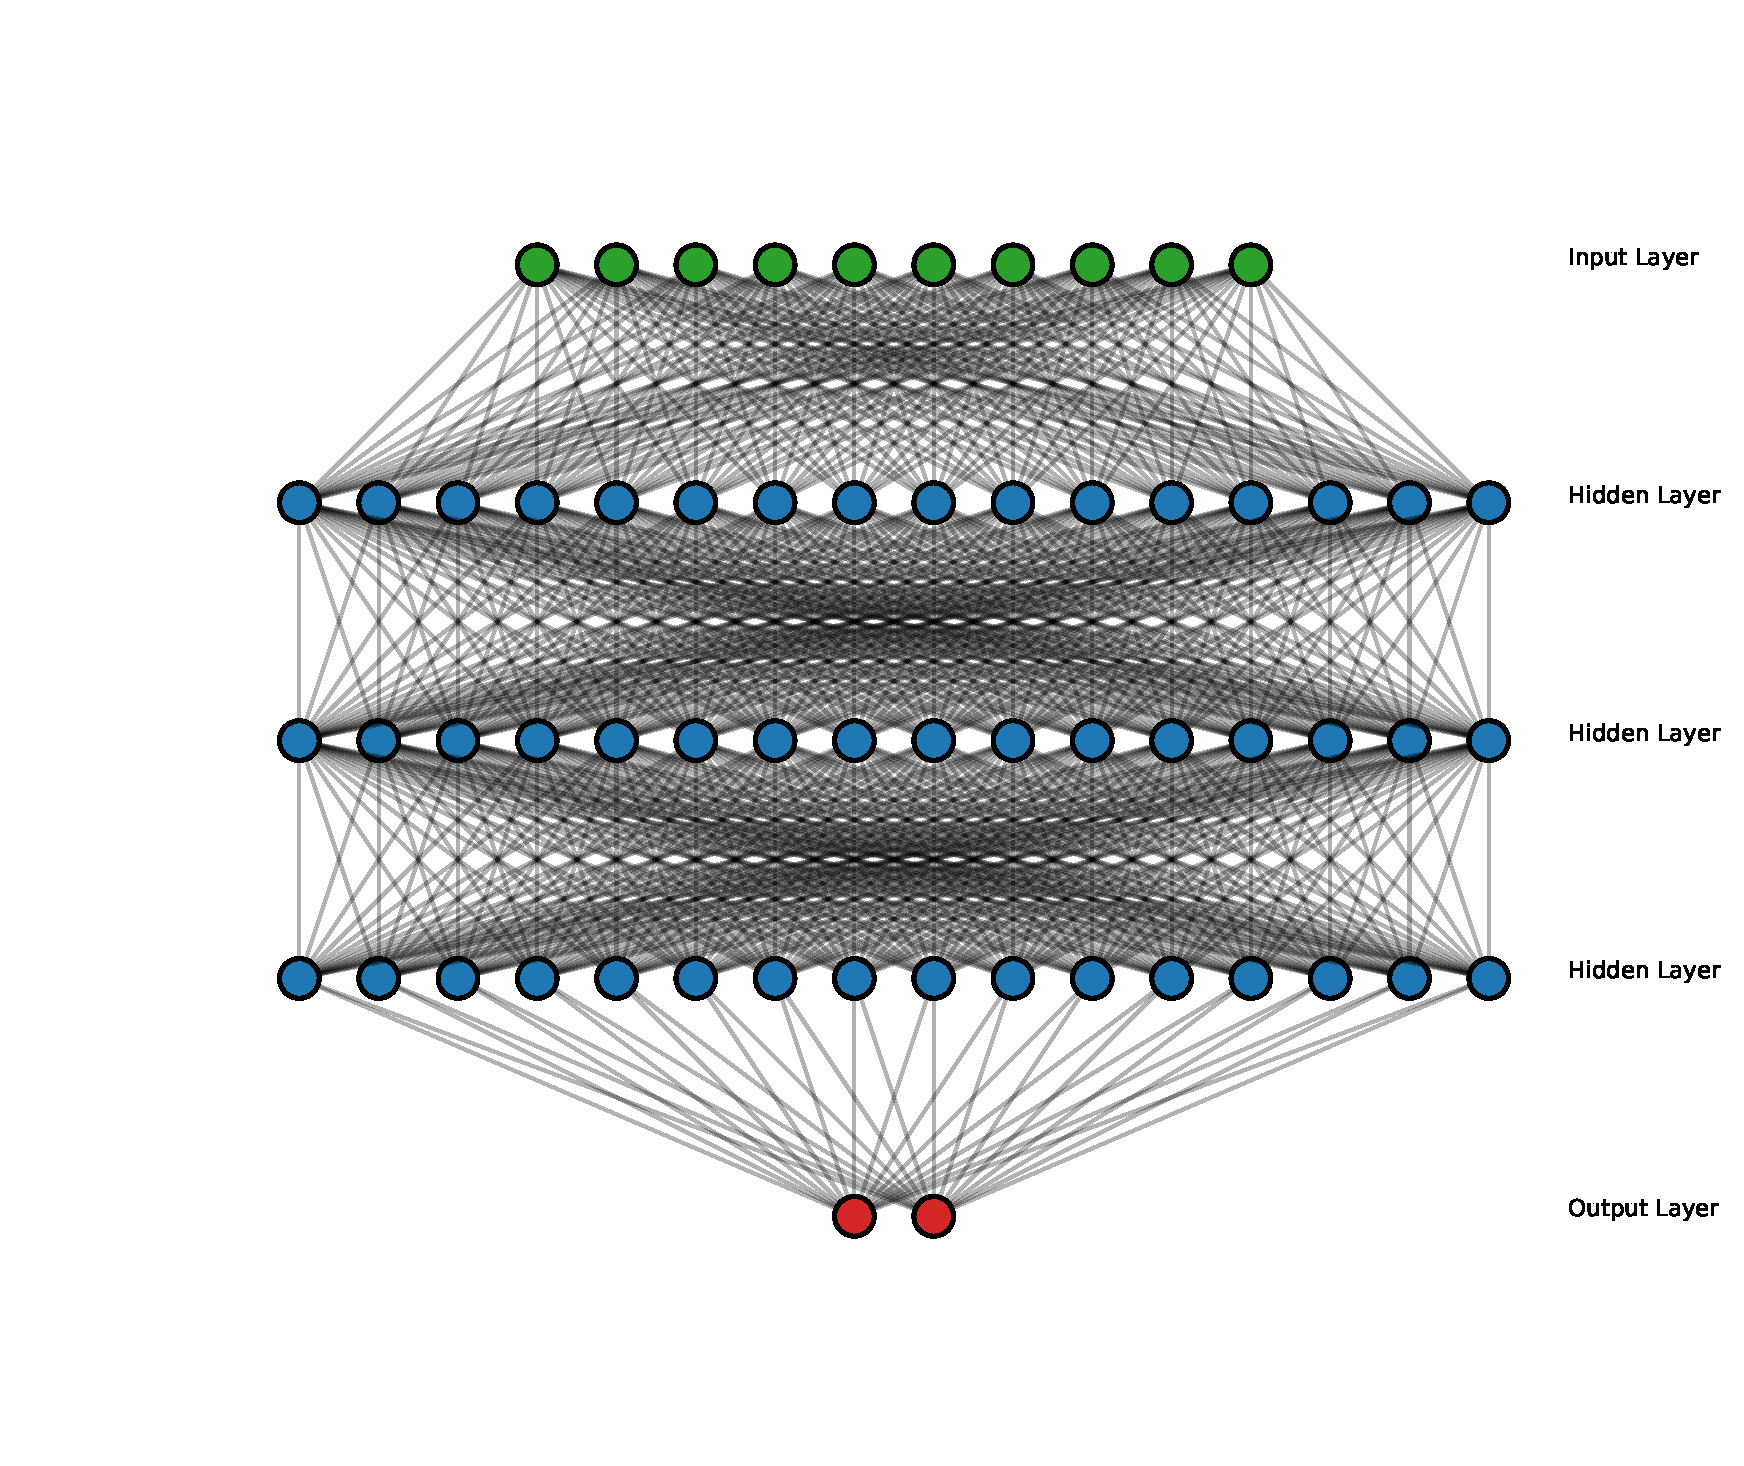
\includegraphics[width=\textwidth]{neuralNetImage}
	\caption{Architektur Neuronales Netz für die NextStep Prädiktion}
	% \todo{Quelle Bild!}
	\label{fig:netArchitectureNextStep}
\end{figure}

% \input{NeuralNet.pgf}

\begin{figure}[h]
    \centering
    \missingfigure{Grafik architektur Separator}
	% 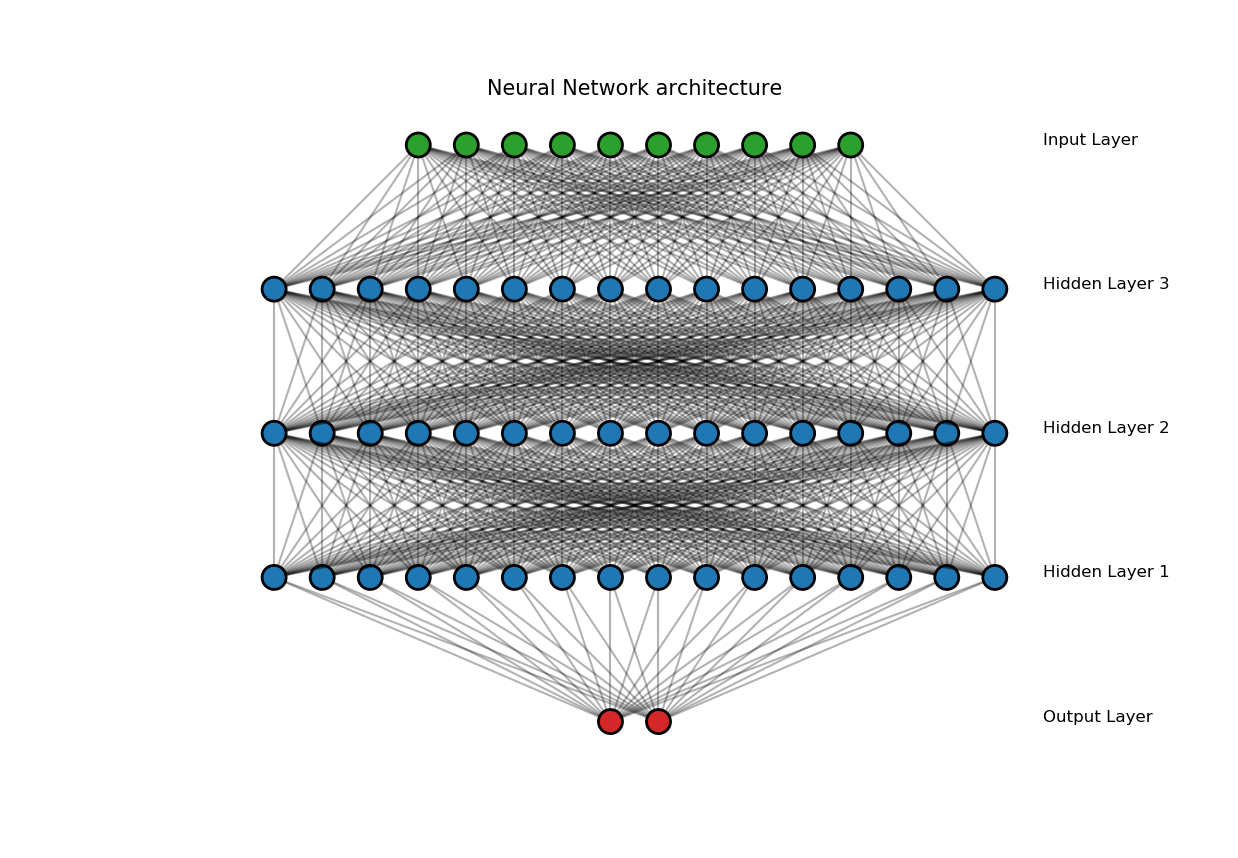
\includegraphics[width=\textwidth]{NN_NextStep_v2}
	\caption{Architektur Neuronales Netz für die Separator Prädiktion}
	% \todo{Quelle Bild!}
	\label{fig:netArchitectureSep}
\end{figure}
